\documentclass[14pt]{beamer}
\usepackage[utf8]{inputenc}
\usepackage{polski}

\usetheme[height=1cm]{Rochester}
\usecolortheme[RGB={0,156,201}]{structure}
\usefonttheme{professionalfonts}
\setbeamertemplate{navigation symbols}{}

\title{Monady w programowaniu funkcyjnym}
\author{Łukasz Dąbek}

\begin{document}

\begin{frame}[plain]
    \titlepage
\end{frame}

\begin{frame}{Samouczki}
    \begin{center}
        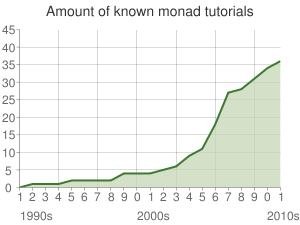
\includegraphics[scale=0.5]{monads-timeline.png}
    \end{center}
\end{frame}

\begin{frame}{Zwięzła definicja}
    \begin{quote}
        A monad is just a monoid in the category of endofuctors,
        what's the problem?
        \vskip5mm
        \hspace*\fill{\small--- Philip Wadler} 
    \end{quote}
\end{frame}


\begin{frame}{Funkcje debugowalne}
    \begin{itemize}
        \item Debugowanie w języku nieczystym jest proste
            (\texttt{printf} w dowolnym miejscu).
        \pause
        \item Jak poradzić sobie w Haskellu?
    \end{itemize}
\end{frame}

\begin{frame}{Funkcje debugowalne}
    \texttt{f, g :: Float -> Float}
    \pause

    \texttt{f x = x + 4}

    \texttt{g x = x * 2}

    \texttt{(f . g) 19 = 42}
\end{frame}

\begin{frame}{Funkcje debugowalne}
    \texttt{f', g' :: Float -> (Float, \emph{String})}
    \pause

    \texttt{f' x = (x + 4, "f was called")}

    \texttt{g' x = (x * 2, "g " ++ show x)}

    \texttt{g' . f' -- błąd typów!}
\end{frame}

\begin{frame}{Kompozycja}
    \begin{itemize}
        \item Chcemy prześledzić wykonanie złożenia funkcji \texttt{f'}
            i \texttt{g'}.
        \item Złożenie \texttt{f} i \texttt{g} to \texttt{f . g}.
        \item Jak złożyć \texttt{f'} i \texttt{g'}?
    \end{itemize}
\end{frame}

\begin{frame}[fragile]
\frametitle{Kompozycja}
\begin{verbatim}
let (y, s) = g' x
    (z, t) = f' y in (z, s ++ t)
\end{verbatim}
\end{frame}

\begin{frame}{Kompozycja}
    \begin{itemize}
        \item Nie chcemy pisać tego kodu wielokrotnie.
        \item \texttt{bind f' :: (Float,String) -> (Float,String)}
    \end{itemize}
\end{frame}

\begin{frame}[fragile]
\frametitle{Bind}
\begin{verbatim}
bind :: (Float -> (Float,String))
     -> (Float,String)
     -> (Float,String)
\end{verbatim}
\end{frame}

\begin{frame}[fragile]
\frametitle{Bind}
\begin{verbatim}
bind f (x,s) =
  let (y,t) = f x in (y,s ++ t)

comp = bind f . g
\end{verbatim}
\end{frame}

\begin{frame}[fragile]
\frametitle{Unit}
\begin{verbatim}
unit :: Float -> (Float,String)
unit x = (x,"")
\end{verbatim}
\end{frame}

\begin{frame}[fragile]
\frametitle{Unit - przykład dowodu}
\begin{verbatim}
bind unit (a, s)
= bind (\x -> (x,"")) (a,s)
= let (y,t) = (\x -> (x,"")) in (y,s++t)
= (a, s ++ "")
= (a, s)
\end{verbatim}
\end{frame}

\begin{frame}{Funkcje niedebugowalne}
    \begin{itemize}
        \item Jak składać funkcje debugowalne ze zwykłymi?
        \item \texttt{f  :: Float -> Float}
        \item \texttt{lift f :: Float -> (Float,String)}
        \pause
        \item \texttt{lift f = unit . f}
    \end{itemize}
\end{frame}

\begin{frame}{Małe podsumowanie}
    \begin{itemize}
        \item \texttt{type Dbg a = (a,String)}
        \item \texttt{f, g::Float -> Float}
        \item \texttt{f', g'::Float -> Dbg Float}
        \item \texttt{bind::(a -> Dbg b) -> Dbg a -> Dbg b}
        \item \texttt{unit::a -> Dbg a}
    \end{itemize}
\end{frame}


\begin{frame}{Funkcje wielowartościowe}
    Pierwiastek kwadratowy (sześcienny) z dodatniej liczby rzeczywistej
    jest funkcją jednowartościową.
\end{frame}

\begin{frame}{Funkcje wielowartościowe}
    \texttt{sqrt, cbrt :: Float -> Float}
    \pause

    \texttt{sixthRoot = sqrt . cbrt}
\end{frame}

\begin{frame}{Funkcje wielowartościowe}
    W przypadku liczb zespolonych każda niezerowa liczba ma n pierwiastków
    n-tego stopnia.
\end{frame}

\begin{frame}{Funkcje wielowartościowe}
    \texttt{sqrt', cbrt' :: Complex -> [Complex]}
\end{frame}

\begin{frame}{Kompozycja}
    \begin{itemize}
        \item Chcemy złożyć funkcje \texttt{sqrt'} i \texttt{cbrt'}.
        \item Problem: \texttt{sqrt'} nie przyjmuje listy!
    \end{itemize}
\end{frame}

\begin{frame}{Kompozycja}
    \texttt{sixthRoot x = concatMap sqrt' (cbrt' x)}

    \texttt{concatMap :: (a -> [b]) -> [a] -> [b]\\
    concatMap = concat . map}
\end{frame}

\begin{frame}{Bind}
    \begin{itemize}
        \item \texttt{bind$_d$::(a -> Dbg b) -> Dbg a -> Dbg b}
        \item \texttt{concatMap::(a -> [b]) -> [a] -> [b]}
        \item \texttt{bind$_m$ = concatMap}
    \end{itemize}
\end{frame}

\begin{frame}{Monada listowa}
    \begin{itemize}
        \item \texttt{type Mv a = [a]}
        \item \texttt{bind$_m$ = concatMap}
        \item \texttt{unit$_m$ x = [x]}
    \end{itemize}
\end{frame}

\begin{frame}{Monady ogólnie}
    Widzieliśmy przykłady, teraz będzie bardziej abstrakcyjnie.
    Jednak najpierw - funktory.
\end{frame}

\begin{frame}{Funktory}
    \begin{itemize}
        \item Typ danych będący ,,polimorficznym kontenerem''.
        \item Przykładowo: \texttt{Maybe}, \texttt{List}, \texttt{Either}.
    \end{itemize}
\end{frame}

\begin{frame}[fragile]
\frametitle{Funktory}
\begin{verbatim}
class Functor f where
    fmap :: (a -> b) -> (f a -> f b)
\end{verbatim}
\end{frame}

\begin{frame}[fragile]
\frametitle{Funktory - prawa}
\begin{verbatim}
fmap id = id
fmap (f . g) = fmap f . fmap g
\end{verbatim}
\end{frame}

\begin{frame}[fragile]
\frametitle{Lista jako funktor}
\begin{verbatim}
instance Functor ([]) where
    fmap = map
\end{verbatim}
\end{frame}

\begin{frame}[fragile]
\frametitle{Maybe jako funktor}
\begin{verbatim}
instance Functor Maybe where
    fmap f (Just x) = Just (f x)
    fmap f Nothing  = Nothing
\end{verbatim}
\end{frame}

\begin{frame}[fragile]
\frametitle{Para jako funktor}
\begin{verbatim}
instance Functor (a,) where
    fmap f (a,x) = (a,f x)
\end{verbatim}
\end{frame}

\begin{frame}[fragile]
\frametitle{Either jako funktor}
\begin{verbatim}
instance Functor (Either a) where
    fmap f (Left a) = Left a
    fmap f (Right b) = Right (f b)
\end{verbatim}
\end{frame}

\begin{frame}[fragile]
\frametitle{Dwa nietypowe funktory}
\begin{verbatim}
data Identity a = I a
data Const x a = C x

instance Functor Identity where
    fmap f (I a) = I (f a)

instance Functor (Const a) where
    fmap _ (Const a) = Const a
\end{verbatim}
\end{frame}

\begin{frame}{Z czego składa się monada?}
    \begin{itemize}
        \item Typu \texttt{m} będącego funktorem.
        \item Funkcji \texttt{unit :: a -> m a}.
        \item Funkcji\\
            \texttt{bind :: (a -> m b) -> m a -> m b}.
        \pause
        \item (W Haskellu nazywają się one trochę inaczej).
    \end{itemize}
\end{frame}

\begin{frame}[fragile]
\frametitle{Klasa Monad w Haskellu}
\begin{verbatim}
class Monad m where
    -- unit zwany return'em
    return :: a -> m a

    -- bind zwany (>>=)
    (>>=) :: m a -> (a -> m b) -> m b
\end{verbatim}
\end{frame}

\begin{frame}[fragile]
\frametitle{Writer Monad}
\begin{verbatim}
data Writer a = (a, String)
instance Monad Writer where
    return x = (x,"")
    (x,s) >>= f = let (y,t) = f x
                  in (y,s++t)
\end{verbatim}
\end{frame}

\begin{frame}[fragile]
\frametitle{List Monad}
\begin{verbatim}
instance Monad [] where
    return x = [x]
    (>>=) = flip concatMap
\end{verbatim}
\end{frame}

\begin{frame}[fragile]
\frametitle{List Monad}
\begin{verbatim}
solutions = [1..5] >>= \x ->
            [1..5] >>= \y ->
            if x * y `mod` 3 == 0
              then return (x,y)
              else []
\end{verbatim}
\end{frame}

\begin{frame}[fragile]
\frametitle{List Monad}
\begin{verbatim}
solutions = do
    x <- [1..5]
    y <- [1..5]
    if x * y `mod` 3 == 0
      then return (x,y)
      else []
\end{verbatim}
\end{frame}

\begin{frame}[fragile]
\frametitle{Maybe Monad}
\begin{verbatim}
data Maybe a = Just a | Nothing
instance Monad Maybe where
    return = Just
    Just a  >>= f = f a
    Nothing >>= _ = Nothing
\end{verbatim}
\end{frame}

\begin{frame}[fragile]
\frametitle{Maybe Monad}
\begin{verbatim}
father :: Person -> Maybe Person
grandgrandfather x =
  case father x of
    Nothing -> Nothing
    Just f1 -> case father f1 of
      Nothing -> Nothing
      Just f2 -> ...
\end{verbatim}
\end{frame}

\begin{frame}[fragile]
\frametitle{Maybe Monad}
\begin{verbatim}
grandgrandfather x =
  father x  >>= \f1 ->
  father f1 >>= \f2 ->
  father f2 >>= return
\end{verbatim}
\end{frame}

\begin{frame}[fragile]
\frametitle{Maybe Monad}
\begin{verbatim}
grandgrandfather x = do
  f1 <- father x
  f2 <- father f1
  father f2
\end{verbatim}
\end{frame}

\begin{frame}[fragile]
\frametitle{Maybe Monad}
\begin{verbatim}
(>=>) :: (a -> m b)
      -> (b -> m c)
      -> (a -> m c)

f >=> g = \a -> f a >>= g

grandgrandfather =
    father >=> father >=> father
\end{verbatim}
\end{frame}

\begin{frame}[fragile]
\frametitle{Maybe Monad}
\begin{verbatim}
nFather :: Int -> Person -> Maybe Person
nFather n = foldr1 (>=>) (repeat n father)
\end{verbatim}
\end{frame}

\begin{frame}{Monoid w kategorii...}
    \begin{itemize}
        \item \texttt{>=>} składa funkcje monadyczne.
        \item Można zdefiniować go w terminach \texttt{>>=}.
        \item \texttt{f >=> g = \char`\\x -> f x >>= g}
    \end{itemize}
\end{frame}

\begin{frame}{Prawa monadyczne}
    \begin{itemize}
        \item \texttt{return >=> f = f}
        \item \texttt{f >=> return = f}
        \item \texttt{a >=> (b >=> c) = (a >=> b) >=> c}
        \pause
        \item Monoid! Operacja łączna z elementem neutralnym.
        \item (\texttt{g :: Functor f => a -> f b} nazywamy endofunktorem)
    \end{itemize}
\end{frame}

\begin{frame}{Prawa monadyczne inaczej}
    \begin{itemize}
        \item \texttt{m >>= return = m}
        \item \texttt{return x >>= f = f x}
        \item \texttt{(a >>= b) >>= c =\\
            a >>= (\char`\\x -> b x >>= c)}
    \end{itemize}
\end{frame}

\begin{frame}{Więcej przykładów}
    Obejrzymy jeszcze kilka przykładów monad i typowych zastosowań.

    Następnie opowiemy o zastosowaniach mniej typowych.
\end{frame}

\begin{frame}[fragile]
\frametitle{Either Monad}
\begin{verbatim}
data Either a b = Left a | Right b
instance Monad (Either a) where
    return = Right
    Left a  >>= _ = Left a
    Right b >>= f = f b
\end{verbatim}
\end{frame}

\begin{frame}[fragile]
\frametitle{Either Monad}
\begin{verbatim}
catch :: Either a b
      -> (b -> Either a b)
      -> Either a b

catch (Left a) handler = handler a
catch (Right b) _ = Right b
\end{verbatim}
\end{frame}

\begin{frame}[fragile]
\frametitle{Either Monad}
\begin{verbatim}
integrate :: Either String Float
solution :: Either String String

solution = 
  (integrate >>= 
    (\f -> return $ "Result: " ++ show f))
  `catch`
  (\s -> return $ "Error: " ++ s)
\end{verbatim}
\end{frame}

\begin{frame}[fragile]
\frametitle{State Monad}
\begin{verbatim}
data State s a = State (s -> (a,s))

instance Monad (State s) where
    return x = \s -> (x,s)
    (State f) >>= g = \s ->
      let (a,s')   = f s
          State g' = g a
      in g' s'
\end{verbatim}
\end{frame}

\begin{frame}[fragile]
\frametitle{State Monad}
\begin{verbatim}
runState (State f) s = f s
get :: State s s
get = State $ \s -> (s,s)

set :: s -> State s ()
set s = State $ \_ -> ((),s)

inc :: State Int ()
inc = do
    s <- get
    set (s + 1)
\end{verbatim}
\end{frame}

\begin{frame}[fragile]
\frametitle{State Monad}
\begin{verbatim}
getRandom :: State Seed Int
getRandom = do
    seed <- get
    let (n, seed') = fromSeed seed
    set seed'
    return n
\end{verbatim}
\end{frame}

\begin{frame}[fragile]
\frametitle{State Monad}
\begin{verbatim}
getOne :: [a] -> State Seed a
getOne xs = do
    rand <- getRandom
    return xs !! (rand `mod` length xs)
\end{verbatim}
\end{frame}

\begin{frame}[fragile]
\frametitle{State Monad}
\begin{verbatim}
example :: State Seed Int
example = do
    a <- getOne [0..10]
    b <- getOne [0..10]
    c <- getOne [0..10]
    return (a + b + c)

runState example initialSeed
\end{verbatim}
\end{frame}

\begin{frame}[fragile]
\frametitle{State Monad}
\begin{verbatim}
nCoins :: Int -> State Seed Int
nCoins n = fmap sum $ sequence 
             (replicate n (getOne [0,1]))

sequence :: Monad m => [m a] -> m [a]
sequence [] = []
sequence (m:ms) = do
    x <- m
    xs <- sequence ms
    return (x:xs)
\end{verbatim}
\end{frame}

\begin{frame}{Podstawowe monady - podsumowanie}
    \begin{itemize}
        \item Monady to ,,design pattern'' programowania funkcyjnego.
        \item Pozwalają operować na jednym z elementów pudełka (funktora) bez
            znajomości jego struktury (\texttt{>>=}).
        \item Pozwalają na modelowanie efektów w czystym języku funkcyjnym (np. stanu).
    \end{itemize}
\end{frame}

\begin{frame}{Tablica}
    Reszta klasycznie - na tablicy.

    W międzyczasie: pytania?
\end{frame}

\begin{frame}
    NULL
\end{frame}

\begin{frame}
    To juz koniec. Dziękuję.
\end{frame}

\end{document}
